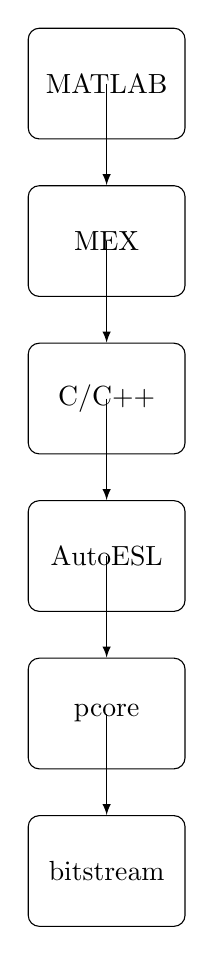
\begin{tikzpicture}[
        >=latex,
        block/.style = {
            rectangle,
            draw,
            text width = 5em,
            text centered,
            rounded corners,
            minimum height = 4em},
        arrow/.style = {
            draw,
            ->,
            -latex},
        node distance = 2cm]
    % Place nodes
    \node [block]                   (matlab)    {\progLang{MATLAB}};
    \node [block, below of=matlab]  (mex)       {\progLang{MEX}};
    \node [block, below of=mex]     (cpp)       {\progLang{C/C++}};
    \node [block, below of=cpp]     (autoesl)   {\software{AutoESL}};
    \node [block, below of=autoesl] (pcore)     {pcore};
    \node [block, below of=pcore]   (bitstream) {bitstream};

    % Edges
    \path [arrow] (matlab)  -| (mex);
    \path [arrow] (mex)     -| (cpp);
    \path [arrow] (cpp)     -| (autoesl);
    \path [arrow] (autoesl) -| (pcore);
    \path [arrow] (pcore)   -| (bitstream);
\end{tikzpicture}